%!TEX root = ../thesis.tex

\section{関連研究}
QDDモータの特徴に着目した研究事例として,Gealyらの「Blue」とZhaoらのQDDロボットアームが挙げられる.\cite{gealy2019quasidirectdrivelowcostcompliant}\cite{10106520}
\subsection{Gealyらの研究: Blueロボットアーム}
Gealyらの研究では,7自由度のロボットアーム「Blue」を開発し,家庭や研究環境での利用を目的とした設計がなされている.(図\ref{fig:blue}参照)このアームはQDDモータを採用し,高いバックドライバビリティを実現することで,物体や人との衝突時のダメージを軽減する構造となっている.さらに,タイミングベルト駆動を採用することで構造を簡素化し,製造コストを約5000ドル以下に抑えている.これにより,柔軟な力制御を実現する低コストなロボットアームとしての可能性が示された.

また,Zhaoらの研究では,モバイルプラットフォームへの搭載を視野に入れた軽量ロボットアームが提案されている.(図\ref{fig:qddarm}参照)このアームは5自由度構成であり,QDDモータの高いバックドライバビリティを活用しながら,トポロジー最適化やアルミニウム合金,樹脂3Dプリント部品を組み合わせて軽量化を図っている.さらに,ピックアンドプレースタスクを想定した実験により,高い柔軟性と安全性を実証している.

これらの研究はいずれも,QDDモータの特徴である高いバックドライバビリティを活かした安全性や柔軟性の向上を目指している点で重要である.しかし,オフィス環境を考慮した設計や,研究者や開発者が容易に利用可能なオープンプラットフォームの実現には至っていない.本研究では,オフィス環境に適応可能なQDDモータ搭載のロボットアームを設計することを目指す.さらに,設計データを公開することで,QDDモータの普及および技術発展に貢献することを期待する.

\begin{figure}[h]
  \centering
  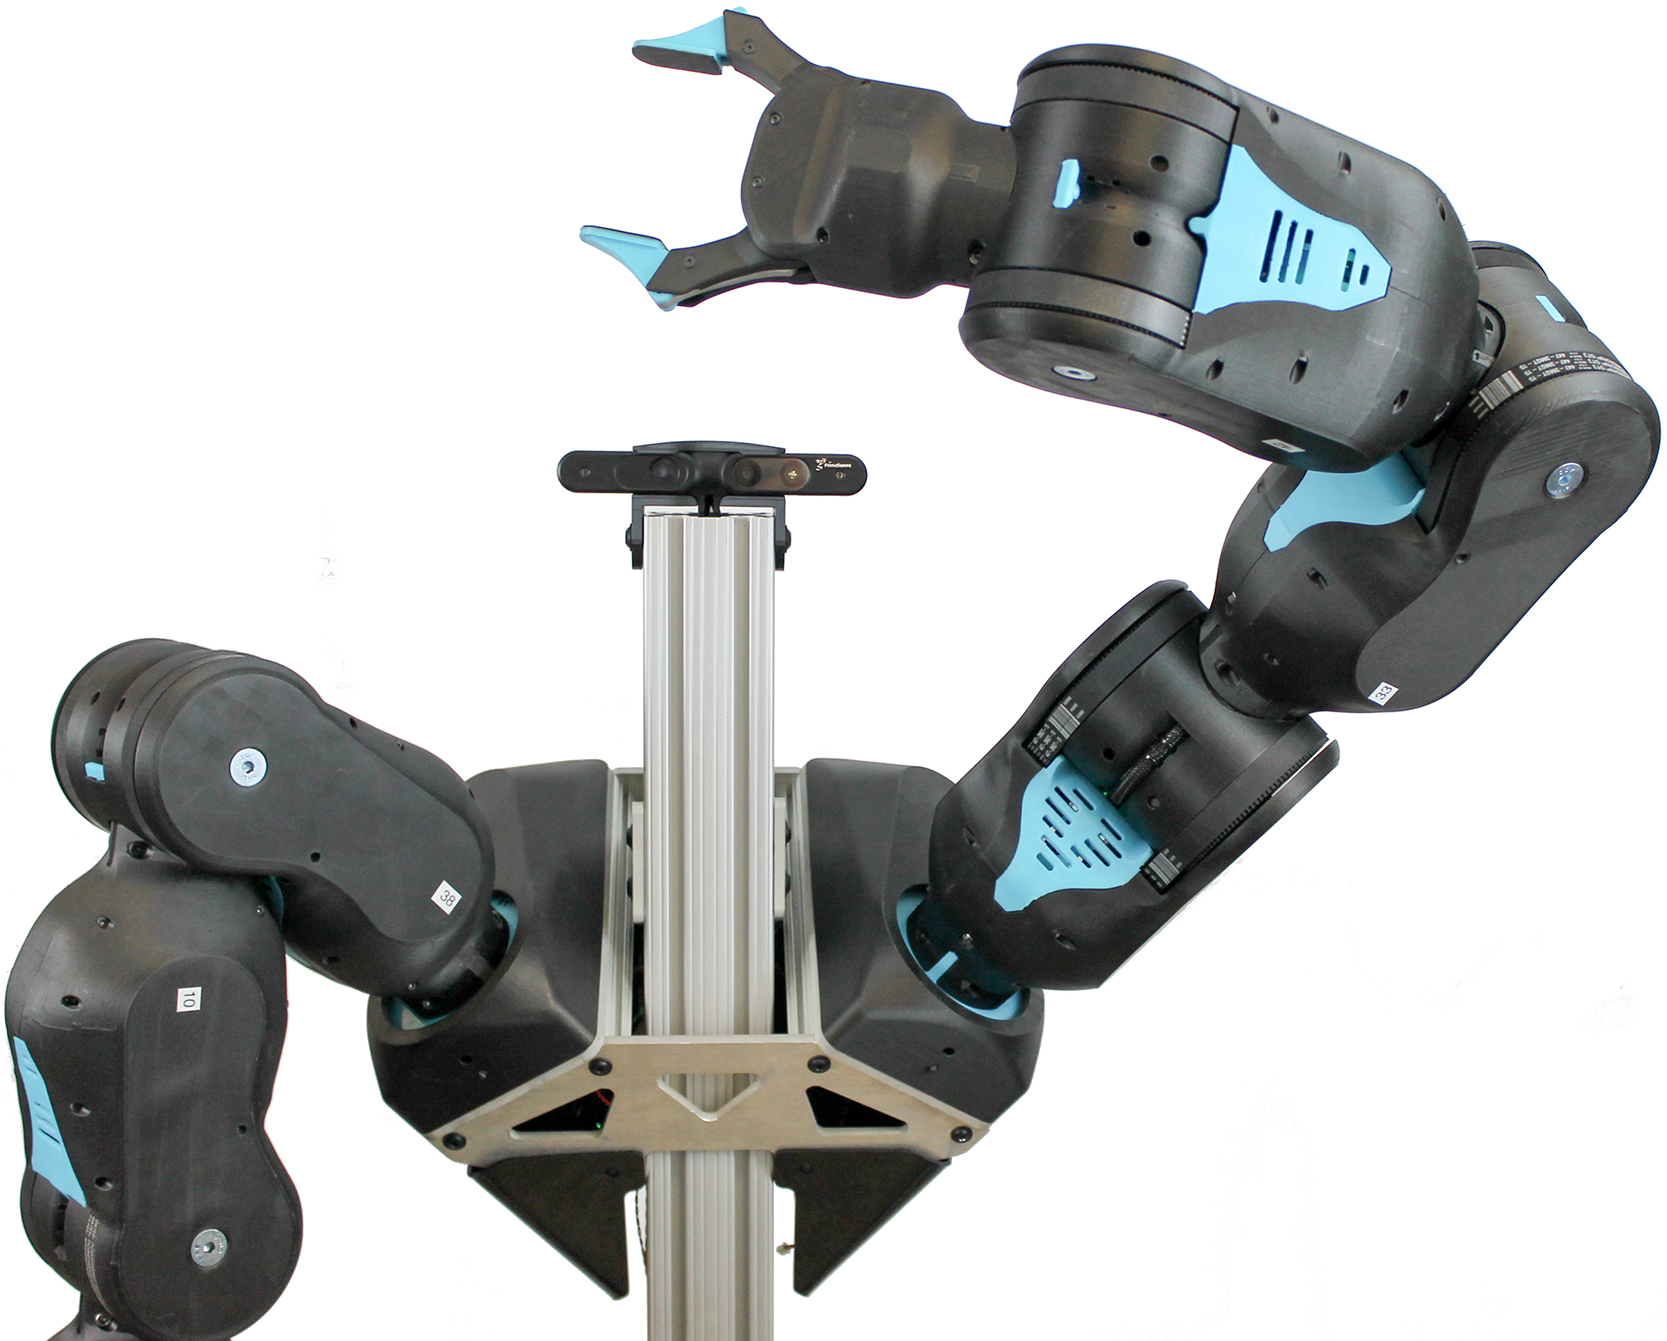
\includegraphics[width=10cm]{images/twoArmTeaser.jpg}
  \caption{The Blue robot arm. (source: \cite{gealy2019quasidirectdrivelowcostcompliant})}
  \label{fig:blue}
\end{figure}

\begin{figure}[h]
  \centering
  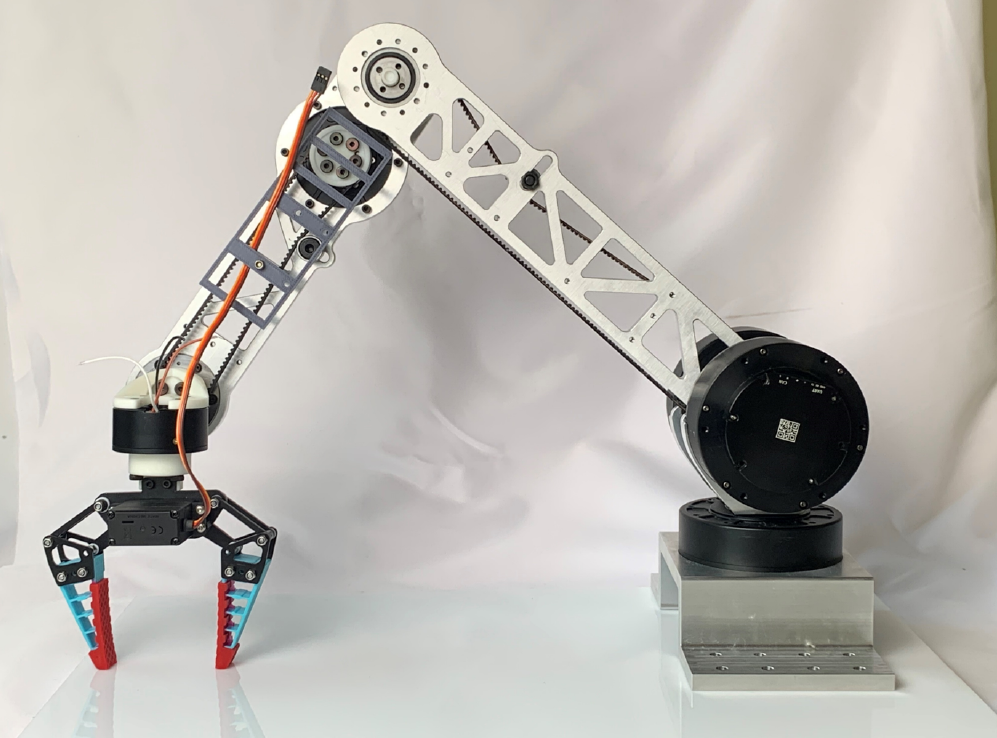
\includegraphics[width=10cm]{images/qddarm.png}
  \caption{The proposed 5-DOF articulated quasi-direct drive (QDD) robot arm,
  together with a commercial 1-DOF soft gripper. (source: \cite{10106520})}
  \label{fig:qddarm}
\end{figure}
\clearpage
\newpage